% !TeX root = ../../main.tex
\newpage
\section{Wyniki z~użyciem sieci Mask R-CNN}

Przedstawione dalej wyniki dotyczą zbioru \textit{low}.
Korzystając z faktu, iż wszystkie obrazy w tym zbiorze są tej samej rozdzielczości 896x640 pikseli, a co za tym idzie każdy składa się z identycznej liczby pikseli w sumie, wynik sieci można w miarodajny sposób porównać między różnymi obrazami licząc poprawnie zidentyfikowane piksele maski. \\
Dla danego obrazu i przewidzianej przez sieć maski, każdy piksel można zaklasyfikować do jednej z następujących kategorii:

\begin{itemize}
  \item True Positive - piksel został poprawnie zakwalifikowany jako powierzchnia kortu;
  \item False Positive - piksel nie wchodzący w powierzchnię kortu został niepoprawnie oznaczony jako powierzchnia kortu;
  \item False Negative - piksel kortu został niepoprawnie zakwalifikowany jako nie wchodzący w powierzchnię kortu;
  \item True Negative - piksel został poprawnie zakwalifikowany jako nie wchodzący w powierzchnię kortu.
\end{itemize}

\begin{figure}[!htb]
  \minipage{0.45\textwidth}
    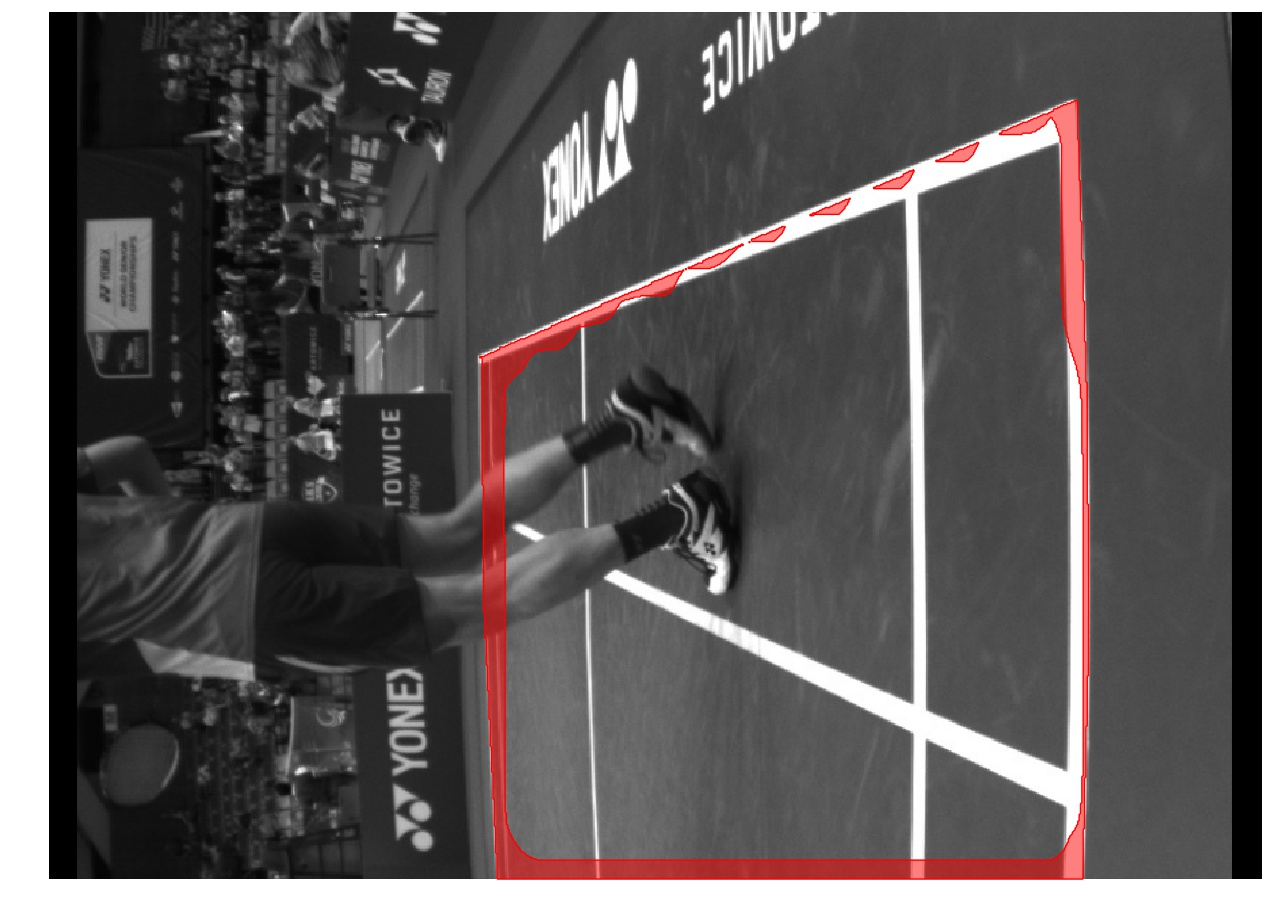
\includegraphics[width=\linewidth]{original_fn_1564911595553287247.jpg}
    \caption{Poglądowy obraz z zaznaczonym obszarem False Negative}
  \endminipage\hfill
  \minipage{0.45\textwidth}
    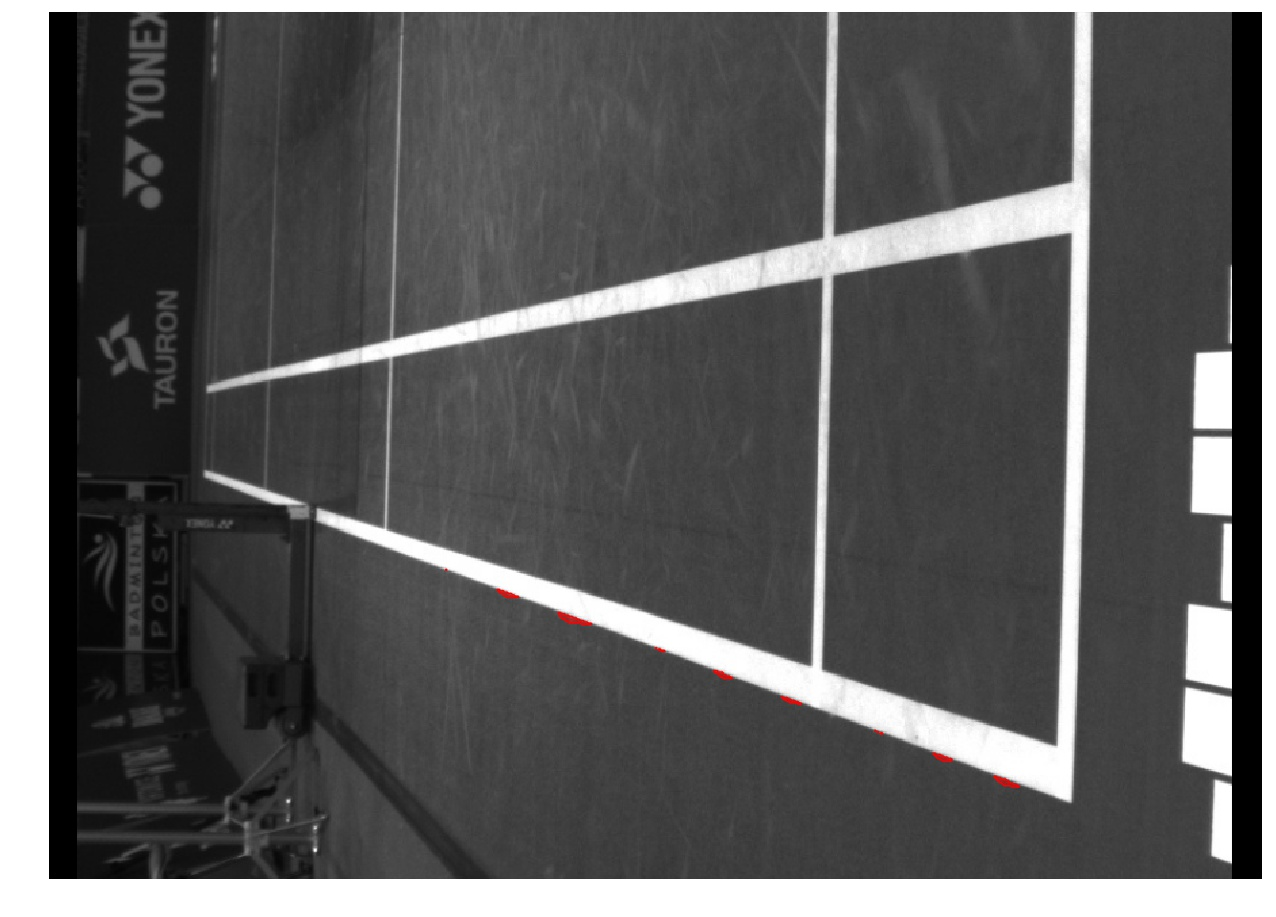
\includegraphics[width=\linewidth]{original_fp_1564953159296706208_5.jpg}
    \caption{Poglądowy obraz z zaznaczonym obszarem False Positive}
  \endminipage\hfill
\end{figure}

\newpage

Wyniki powyższej klasyfikacji przedstawiają się następująco. Wartości procentowe odnoszą się do liczby pikseli w sumie na obrazach, czyli 573440 pikseli.

\begin{table}[!h]
	\centering
	\caption{Wyniki na zbiorze \textit{low}}
	\vspace{6pt}
	{\footnotesize
		\begin{tabular}{|c|c|c|c|c|}
			\hline \textbackslash & True Positive & False Positive & False Negative & True Negative \\
      \hline Średnia & 270830.84 (47.23\%) & 131.63 (0.02\%) & 21976.08 (3.83\%) & 280501.45 (48.92\%) \\
      \hline Minimum & 147267 (25.68\%) & 0 (0.0\%) & 10954 (1.91\%) & 63840 (11.13\%) \\
      \hline Maksimum & 488682 (85.22\%) & 668 (0.12\%) & 53684 (9.36\%) & 414944 (72.36\%) \\
      \hline Mediana & 265394.0 (46.28\%) & 87.0 (0.02\%) & 21166.0 (3.69\%) & 285509.0 (49.79\%) \\
      \hline
		\end{tabular}
	}
	\vspace{0pt}
\end{table}

\vspace{1cm}

Z powyższych wyników można obliczyć następujące metryki:

\begin{itemize}
  \item Accuracy - $ \frac{TP + TN}{TP + TN + FP + FN} $,
  \item Sensitivity - $ \frac{TP}{TP + FN} $,
  \item Specificity - $ \frac{TN}{TN + FP} $,
  \item Precision - $ \frac{TP}{TP + FP} $;
\end{itemize}

Obliczone metryki zostały przedstawione w następującej tabeli:

\begin{table}[!h]
	\centering
	\caption{Obliczone metryki na zbiorze \textit{low}}
	\vspace{6pt}
	{\footnotesize
		\begin{tabular}{|c|c|c|c|c|}
			\hline \textbackslash & Accuracy & Sensitivity & Specificity & Precision \\
      \hline Średnia & 0.96 & 0.92 & 1.0 & 1.0 \\
      \hline Minimum & 0.91 & 0.88 & 1.0 & 1.0 \\
      \hline Maksimum & 0.98 & 0.96 & 1.0 & 1.0 \\
      \hline Mediana & 0.96 & 0.93 & 1.0 & 1.0 \\
      \hline
		\end{tabular}
	}
	\vspace{0pt}
\end{table}
